\documentclass[11pt]{article}
\usepackage[usenames, dvipsnames]{color}
\definecolor{pass_grn}{RGB}{0, 230, 0}
\definecolor{fail_red}{RGB}{230, 0, 0}
\usepackage{fancyhdr}
\usepackage[a4paper, total={6in, 8in}]{geometry}
\usepackage{graphicx}
\usepackage{multirow}
\usepackage{pifont}
\newcommand{\cmark}{\ding{51}}%
\newcommand{\xmark}{\ding{55}}
\usepackage{subcaption}
\usepackage{titling}
\usepackage[nottoc,numbib]{tocbibind}
\usepackage{wrapfig}
\pagestyle{fancy}
\fancyhead{}
\renewcommand{\headrulewidth}{0pt}
\fancyfoot[LE,RO]{Y1481702}
\newcommand{\myparagraph}[1]{\paragraph{#1}\mbox{}\\}

\title{Software Testing}
\author{Y1481702}
\date{\today}
\setlength\parindent{0pt}

%\setlength{\droptitle}{-2em} %ADJUST HEIGHT OF TITLE
%\addtocontents{toc}{\protect\setcounter{tocdepth}{2}} %ADJUST WHICH SECTIONS APPEAR IN CONTENTS TABLE

\begin{document}
\begin{titlepage}
\clearpage\maketitle
\thispagestyle{empty}
\tableofcontents
\end{titlepage}

%Your report must not exceed 10 sides of A4, minimum of 11pt font
%minimum 120% line spacing
%o: correct, see https://tex.stackexchange.com/questions/348678/how-to-set-document-line-spacing-in-pt-format
%minimum 2cm margins on all sides

%does not include covering page, table of contents or reference list

%EXAM NUMBER SHOULD BE WRITTEN ON THE FRONT PAGE AND ALL SUBSEQUENT PAGES
%APPROX ONE PAGE PER 10 MARKS:


%GENERAL ADVICE:
	%You won’t receive marks for testing that the marker merely thinks you probably did — marks will only be awarded for tests that are described explicitly and precisely.
	%Yes, it is a little unrealistic that you are only allowed 10 pages and 8 tests, and that your possible coverage and comprehensiveness are limited by that. However, in the real world there are always resource limits — the ones you have here are merely artificial ones.
	%Do not repeat anything that does not vary. For example, do not repeat the same boilerplate text in every test case description — if something is true for all test cases, say this once at the start of the section.
	%Similarly, use blanket statements to make points that are true of multiple (but not all) tests case (e.g. “Test cases 1–5 assume that...”)
	%Appendices containing full JUnit code or detailed test output etc are not required and will not be read.
	%In general, do not waste space on spurious information. Think about what the notional target reader needs to know in order to use your document, and include only that. At best, other information will waste some of the limited pages available to you.
	%If you reference an external document (such as the documentation or website for the software you are testing), be sure to cite it appropriately, just as in any other submitted work.

\section{Test Plan}% 25 Marks (2.5 pages)
%A test plan
%It should detain the methods used to build the test cases and the software tools used to achieve these
\subsection{Introduction}
%o: What is JAVA MASON?
MASON is a software library for creating agent-based simulations in Java. 
%o: From a testing point of view MASON is a form of OPEN SOURCE SHRINKWRAP
	%may be used in the wild by many people
	%what other ramifications does this have
The software fits into the category of shrinkwrap meaning it might be in use in a wide range of real-world production environments. The software is freely-available and open-source, which is a special case of shrinkwrap software. A common trait of open-source software is that tasks 'that are not considered "fun" often don't get done'.\cite{five_worlds}
%As open source software is often developed without anyone being paid,
	%only "fun" things are done
	%i.e. NOT TESTING
For MASON in particular, it is likely that the software has not been thoroughly tested as there is no trace of any automated testing, either on the MASON website, or its GitHub repository.

%usage statistics can provide with an estimate of how well it needs to work
%biological simulations- high profile studies have based hypotheses on this framework

\subsubsection{Tools}
The IntelliJ IDE was used to explore the code and develop automated tests. This IDE gives powerful features, including plugins for generating code metrics and displaying coverage of unit testing.
JUnit has been used to create automated unit testing for the software.
Git version control has been used to manage the code for these JUnit tests.
For a long term project, this would be particularly advantageous as any automated tests could be updated and versioned alongside any future code changes.

\subsection{Test Coverage}
\subsubsection{System Overview}
%Explain the overall strategy you used for creating test cases, and for selecting the specific test cases that you present in section B
In order to design appropriate test cases an understanding of all levels of the system was needed. As resources here are significantly limited, with only 8 testcases are allowed, it will be necessary to ensure they are used in the most effective way.
%Clearly define what constitutes "the software under test" and list the features that you will test and not test
As stated in the project brief, the testing only needs to cover the following packages, but not their subpackages:

\begin{itemize}
\item \texttt{sim.engine} is responsible for the core simulation management, including the agent scheduling.
\item \texttt{sim.field} provides abstract classes for the representations of space in MASON simulation models, with subpackages managing specific instances of these.
\item \texttt{sim.field.grid} provides various 2D and 3D grid representations of simulation space.
\end{itemize}

Each of the Fig. \ref{fig:loc} shows the proportional sizes of each of these three modules.
\\

It has been shown across software projects that some modules of code may be significantly more error prone than others.
The Pareto principle is said to hold with software bugs, with 80\% of software bugs being found within 20\% of the code\cite[pp. 124]{pressman}.
We can use a variety of metrics about our software to predict which parts of the code that these bugs may be hiding in\cite{predicting_from_history}.
\\

%Complexity:
High cyclomatic complexity (Fig. \ref{fig:cc}/Fig. \ref{table:cc}) can be a good indicator of the most bug-ridden sections of applications.
%Dependency:
Fig. \ref{table:dependency} shows how the packages in the test scope interact with other packages in the system. In particular, \texttt{sim.engine} is relied on by a large number of packages.
%IntelliJ's Diagram feature helped to show how different components of the system are connected.
%Code Coverage during simulation/runtime?
Code coverage has provided a good understanding of which parts of the [code] are regularly used while running the software.
%Code changes:
How often different source files have changes is also a particularly useful metric. Files which are subject to frequent change have had more opportunity to develop additional bugs.
%Plot cyclomatic complexity against loc for files?
%files which score high on this are likely to contain bugs- SHOULD BE REFACTORED
\\

%Unavailable?
Producing the right metrics to help test the application have been particularly difficult in this case.
No real history of previous bug tracking
GitHub commits are all credited to \textit{eclab} rather than individual developers
\\

\begin{figure}
\begin{subfigure}[b]{0.5\textwidth}
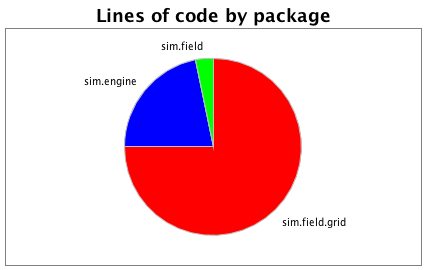
\includegraphics[width=\textwidth]{Appendix/LOC}
\caption{Lines of Code}
\label{fig:loc}
\end{subfigure}
\begin{subfigure}[b]{0.5\textwidth}
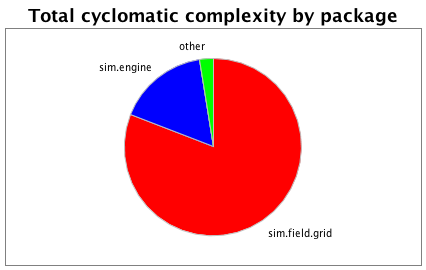
\includegraphics[width=\textwidth]{Appendix/Cyclomatic}
\caption{Cyclomatic Complexity}
\label{fig:cc}
\end{subfigure}

\caption{Charts showing various metrics of MASON}
\label{fig:metric_charts}
\end{figure}

%much of the project is several years old.. why is this?
%	stable to not require updating

%are there any special features of the packages that are notable for testing?
%	UI Testing is hard to test - See Lecture 6
%	OO Code is hard to test
%	concurrency	

%how do we know how a general user works?
%examples of real-world usage (PPSim), vs mason tutorials


\subsubsection{Testing Goals}
%Define acceptability criteria for the software - what (testable) properties does it need to have in order for it to be acceptable quality for its intended purpose?
%o: These will help define the goals of our testing:
	%find the maximum number of bugs?
	%know whether we have undiscovered bugs?
	%o: ^^THIS IS THE MAIN GOAL HERE- 'the institute would like to know if they can really trust the system to be dependable'
	%'want you to provide a thorough assessent of its freedom from defects'
	%comply with regulator-set demands

	%have a compelling defence in a courtcase (self-driving cars, too soon?)
	%minimum time and cost?
		%obviously here we have a set TIME- open assessment for 10 credit module
There are a number of goals we could define for our testing, such as finding the maximum number of bugs or complying with regulator set demands.
The given requirement here is to verify, with a limited number of resources, that the software is dependable.
In general, it's better to test with the aim of showing a product fails, if we cannot do so then the product is reliable enough\cite[pp. 20]{lessons_book}.
As such, the main requirement for our testing is to find any significant undiscovered bugs in commonly used code.
\\

Due to limited resources, the tests will aim to cover the parts of the software which are likely to be used more often by the target users.
MASON is bundled with some demo simulations that give example usages for the library.
Running these simulations with code coverage detection turned on has given a good overview of which parts of the code are used regularly.
Core simulation code that is used routinely by all simulations regardless of their customisations should be tested the most rigourously.
Both the documentation and code coverage checks indicate that this type of code can be found within \texttt{sim.engine}.

\subsubsection{Expected Behaviour}
%usage by a private biological research institute
%users will be research scientists with BASIC Java training
The system behaviour has been tested against the inferred requirements of the client, a private biological research institute.

%Explain how you have determined the expected behaviour of the software (in the absense of an exhaustive and explicit requirements specification)
The expected behaviour of the software has been determined using the extensive MASON documentation\cite{mason_doc}, first-party example implementations as well as a number of open-source examples\cite{ppsim}.

\subsubsection{Unit Testing}
Unit Testing allows the testing of small sections of source code. In this case, unit tests will help us to isolate the select packages that are within the scope of testing from the rest of the system.
\\

Unit testing should focus on core code that is a dependency for other modules, code that regularly gathers bugs and code that is changed by a number of different developers. It should not cover trivial code, such as accessors and mutators, code with non-deterministic results or UI code.\cite{dont_test_blindly}
%Unit Test: sim.engine?
		   %sim.field.. whichever grid is most relevant to biologists?

Mention Pareto principle again!
Aim for 60-70\% code coverage of business logic, %has this come from don't test blindly?
\textasciitilde 20\% of the overall application.

%Mutation Testing?

\subsubsection{System Testing}
%TEST THE WHOLE SYSTEM, typically blackbox
%In this case 'the system is our selected packages'

%Functional, but ALSO non-functional requirements..
	%non-functional requirements:
		%basic Java programming?
		%portability
		%open source

\subsubsection{Integration Testing}
%testing interacting classes..

%not fully within the scope of our testing, we have only been asked to test
	%sim.engine
	%sim.field
	%sim.field.grid

%We CAN/COULD test interacting classes here?

\subsubsection{Acceptance Testing}
Acceptance Testing could be performed to determine if the software can be operated effectively by our end users.
Acceptance testing can be useful for understanding the domain of our software better, but as we are not intending to further develop MASON, this is not particularly relevant here.
%Should be meaningful for the customer- performed on potential users
%-not available as an option due to the requirement to find users...
Acceptance Testing should be performed ON?/BY? domain experts?- I am NOT a domain expert..
\\

While acceptance testing will not help us determine that the software is \textit{dependable}, it would help to discover if it is appropriate for the target audience. In particular, our users have supposedly only received a basic level of Java training. It has been stated that MASON is less-suited to beginner programmers, when compared to other tools, such as NetLogo\cite{abm_platforms_review}.
%BUT NOT PART OF OUR BRIEF, this will be done in a later stage once we decide if the tool is free from defects

%modules in question, aren't directly accessible to the user?

\subsubsection{Regression Testing}
Unfortunately neither the website nor the GitHub repository for MASON provide any previously implemented automated testing.
Either this testing has not been done, which is common with freely-distributed software, or it has not been publicly distributed.
As such, it will not be possible to run any regression testing as part of the project.

\section{Test Case Specifications}% 30 Marks (3 pages)
%Test case specifications for 8 fully specified test cases. The test cases must be complementary: they must make different assumptions and test different specific features of the library.
	%At minimum, each test case should describe the stimulus applied to the software (which might be a sequence of API calls, a sequence of user actions that are taken, or something else) and the expected
		%i.e. correct behaviour
		%N.B. for some tests it may be appropriate to define constraints (e.g. "no files will be changed") instead of/as well as positive statements of behaviour (e.g. "the user will be returned to the main menu screen").
		%Where the reason why the expected/correct behaviour is indeed expected and correct is not obvious to a capable programmer where some domain knowledge, explain briefly why it is so
	%Each test case should also state the purpose of the test within the test set. A good way to do this may be to state the question that the test case asks about the software. If we cannot understand what the purpose of a given test case is, we cannot give you much credit for it.
	%“One test case” should test one thing – one feature, one unusual input, or one user task. For example, if you have a function that takes an integer as an input, testing it with Min/Max/+1/0/-1 should be five test cases. One can note that those are, however, five very low-level (unit test) test cases, which are unlikely to give you the most testing power in a fixed number of tests, and hence unlikely to give you maximum marks.
	%You should aim to provide a diverse range of test cases, and also to provide your best test cases (including any that find interesting bugs). There is an inevitable tension between these two objectives, which you will have to decide how to resolve.
	%For full marks in this section, tests should be conducted at a range of testing levels, including unit, integration and system level. Hint: explicitly label each of your tests with what level it’s working at.
	%You may include short fragments of code within your test case specifications, but not larger ones. In particular, do not include whole JUnit tests. In essence, you need to provide enough information for a smart programmer to recreate your test code given some effort. e.g. if a test case involves a specific sequences of method calls, that sequence of method calls needs to be clear from the test case description.


%o: "Black box testing means that knowledge of the internals of the product doesn't play a significant part in your testing."\cite{lessons_book}
%o: "To do black box testing well, learn about the user, their expectations and needs, the technology and configurations the software will run on, the other software that this software will interact with, the date the software must manage, the development process, and so on. The advantage of black box testing is that you probably think differently than the programmer, and, thus are likely to anticipate risks that the programmer missed."
\subsection{Test Cases 1-3}
\begin{wrapfigure}{r}{0.4\textwidth} 
  \begin{center}
    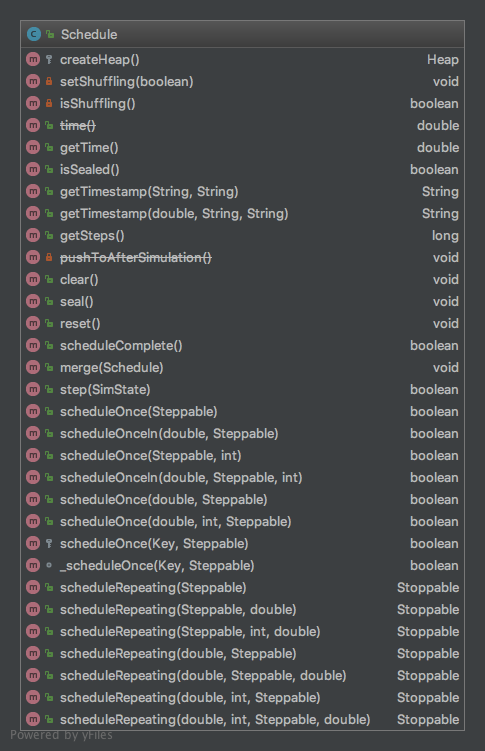
\includegraphics[width=0.4\textwidth]{Appendix/Schedule}
    \caption{Schedule Class}
    \label{fig:schedule}
  \end{center}
\end{wrapfigure}
As previously stated, our initial unit testing will focus on the simulation scheduler which provides the core functionality for MASON. This functionality is contained within the Schedule class as shown in Fig. \ref{fig:schedule}. While this class initially appears to be quite large, at closer inspection, many of its methods are simply overloading others, due to Java's lack of real support for default function arguments.

By removing trivial methods (accessors, mutators, overloading methods), we can reduce the class down to:
\begin{itemize}
	\item \texttt{getTimestamp}: Returns a given time in string format.
	\item \texttt{merge}: Merge a given schedule into this one.
	\item \texttt{step}: Moves the schedule forward by one implementation, skipping empty timesteps.
	\item \texttt{\_scheduleOnce}: Adds the specified item to the schedule, to occur at the specified timestep.
	\item \texttt{scheduleRepeating}: Adds the specified item to the schedule, to repeat continously at specified interval.
\end{itemize}

By constructing a test that ensure the simulation step function works correctly, we will also indirectly test that the schedule method works as expected.


\subsection{Test Case 4}
\subsection{Test Case 5}
\subsection{Test Case 6}
\subsection{Test Case 7}
\subsection{Test Case 8}

\section{Test Results}% 15 marks (1.5 pages)
%The test results for each of the tests that were specified in item B.
	%Here, you should document the results that occurred when the test cases are run. You should provide explicit indication of whether each test passed or failed, and in the latter case state what happened instead.

%o: screenshots may be useful, but add them in appendix?
\begin{center}
\begin{tabular}{|c|c|r|}
	\hline
	\textbf{Test Case} & \textbf{Passed} & \textbf{Description} \\
	\hline
	1 & \textcolor{pass_grn}{\cmark} &\\
	\hline
	2 & \textcolor{fail_red}{\xmark} &\\
	\hline
	3 & \textcolor{pass_grn}{\cmark} &\\
	\hline
	4 & \textcolor{pass_grn}{\cmark} &\\
	\hline
	5 & \textcolor{pass_grn}{\cmark} &\\
	\hline
	6 & \textcolor{pass_grn}{\cmark} &\\
	\hline
	7 & \textcolor{pass_grn}{\cmark} &\\
	\hline
	8 & \textcolor{pass_grn}{\cmark} &\\
	\hline
\end{tabular}
\end{center}

\section{Test Summary Report}% 30 marks (3 pages)
%A test summary report that will contain at least:
	%a summary of the testing that you performed
	%a summary of the results you observed, including a classification of the faults found (by an appropriate classification scheme of your choosing)
	%an overall evaluation of the thoroughness and quality of the testing you have performed
		%o: code coverage results for unit testing?
		%This should be in terms of what might be possible given substantial resources, not in terms of what is possible in a project with this time allocation and maximum report length.
		%Describe the branch coverage and condition coverage, or the mutation score according to a reasonable mutation testing approach, that your tests achieved of the Java code (not of any other artefact). Briefly explain how you did it; make sure you state what tools you used and (where applicable) what mutation operators you used.
	%an overall evaluation of the software tested (in terms of its freedom from faults)
		%o: obviously due to time and limitations on the number of test cases, this is a limited assessment
		%o: but OVERALL..?

The significant limitations of testing resources reduce the level of confidence with which we can say that the software is free from defects.

%Throughout, the summary report should only refer to the test cases that were specified in (B), not any other testing you may have performed.

\newpage
\raggedright
\bibliography{Report}{}
\bibliographystyle{ieeetran}
\newpage
\section{Appendix}

%CODE METRICS:
%Courtesy of the MetricsReloaded IntelliJ plugin:
%MAY WANT TO MOVE some of these tables into the report body if relevant?

\begin{figure}[htp]
\begin{subfigure}[b]{0.5\textwidth}
\begin{center}
\begin{tabular}{|c|r|}
	\hline
	\textbf{Package} & \textbf{Lines of Code} \\
	\hline
	\texttt{sim.engine} & 2,961 \\
	\texttt{sim.field} & 444 \\
	\texttt{sim.field.grid} & 10,248 \\
	\hline
	\textbf{Total} & 13,653 \\
	\hline
	Average & 4,551 \\
	\hline
\end{tabular}
\end{center}
\caption{Lines of Code}
\label{table:loc}
\end{subfigure}
\begin{subfigure}[b]{0.5\textwidth}
\begin{center}
\begin{tabular}{|c|r|}
	\hline
	\textbf{Package} & \textbf{Class Count} \\
	\hline
	\texttt{sim.engine} & 25 \\
	\texttt{sim.field} & 6 \\
	\texttt{sim.field.grid} & 14 \\
	\hline
	\textbf{Total} & 45 \\
	\hline
	Average & 15 \\
	\hline
\end{tabular}
\end{center}
\caption{Class Count}
\label{table:class_count}
\end{subfigure}

\par\bigskip

\begin{subfigure}[b]{0.5\textwidth}
\begin{center}
\begin{tabular}{|c|r|r|}
	\hline
	\multirow{2}{4em}{\textbf{Package}} & \multicolumn{2}{|c|}{\textbf{v(G)}} \\
	\cline{2-3}
	& Average & Total \\
	\hline
	\texttt{sim.engine} & 2.43 & 374 \\
	\texttt{sim.field} & 2.38 & 57 \\
	\texttt{sim.field.grid} & 3.75 & 1,829 \\
	\hline
	\textbf{Total} && 2,260 \\
	\hline
	Average & 3.39 & 753.33 \\
	\hline
\end{tabular}
\end{center}
\caption{Cyclomatic Complexity}
\label{table:cc}
\end{subfigure}
\begin{subfigure}[b]{0.5\textwidth}
\begin{center}
\begin{tabular}{|c|r|r|}
	\hline
	\textbf{Package} & \textbf{Dependencies} & \textbf{Dependants} \\
	\hline
	\texttt{sim.engine} & 2 & 54 \\
	\texttt{sim.field} & 1 & 24 \\
	\texttt{sim.field.grid} & 2 & 20 \\
	\hline
	Average & 1.67 & 32.67 \\
	\hline
\end{tabular}
\end{center}
\caption{Package Dependency}
\label{table:dependency}
\end{subfigure}

\caption{Code Metrics for the relevant MASON libraries}
\label{tables:metrics}
\end{figure}

\begin{figure}[htp]
\centering
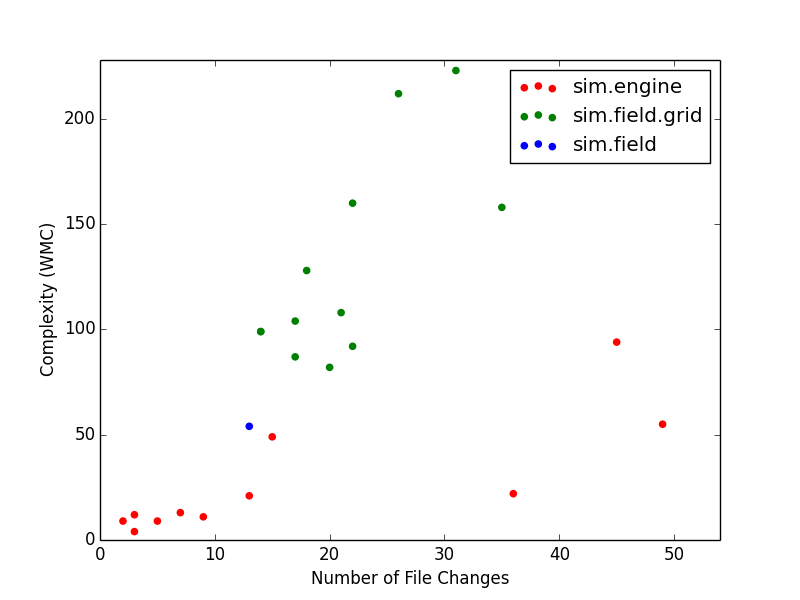
\includegraphics[width=\textwidth]{Appendix/complexityVchange}
\caption{Cyclomatic Complexity and Number of File Revisions for classes in Test Scope}
\label{fig:complexityVchange}
\end{figure}

\begin{figure}[htp]
\centering
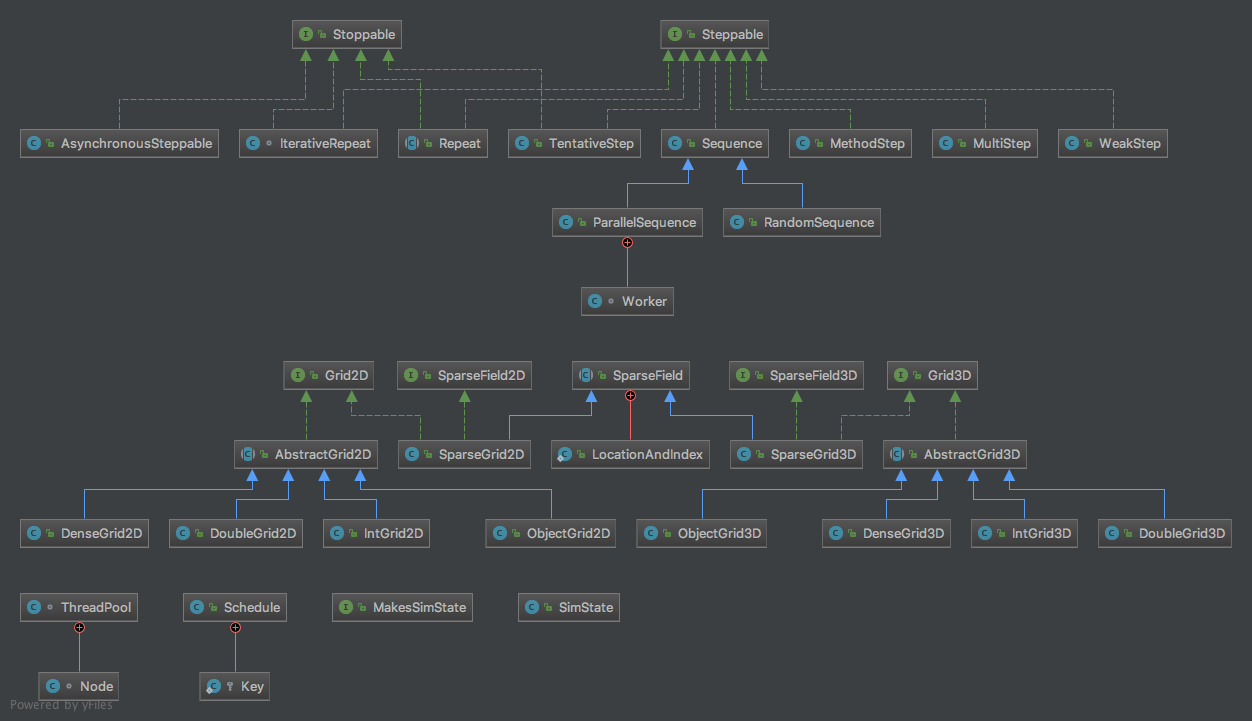
\includegraphics[width=\textwidth]{Appendix/UML}
\caption{Reverse Engineered UML diagram of Class Hierarchy}
\label{fig:uml}
\end{figure}

\begin{figure}[htp]
\begin{center}
\begin{tabular}{|l|l|r|r|r|r|}
	\hline
	\multirow{3}{7.5em}{\textbf{Package}} & \multirow{3}{4em}{\textbf{Class}} & \multicolumn{2}{|p{3cm}|}{\textbf{HeatBugs\newline Coverage (\%)}} & \multicolumn{2}{|p{3cm}|}{\textbf{Virus Infection\newline Coverage (\%)}} \\
	\cline{3-6}
	&& Method & Line & Method & Line\\
	\hline
	\multirow{13}{6em}{\texttt{sim.engine}}
	& AsynchronousSteppable & & & & \\
	& IterativeRepeat & 60 & 70 & 60 & 70 \\
	& MethodStep & & & & \\
	& MultiStep & & & & \\
	& ParallelSequence & 38 & 59 & & \\
	& RandomSequence & & & & \\
	& Repeat & & & & \\
	& Schedule & 41 & 51 & 41 & 50 \\
	& Sequence & 11 & 12 & & \\
	& SimState & 31 & 18 & 31 & 18 \\
	& TentativeStep & & & & \\
	& ThreadPool & 66 & 76 & & \\
	& WeakStep & & & & \\
	\hline
	\texttt{sim.field} & SparseField & 21 & 34 & 21 & 35 \\
	\hline
	\multirow{12}{6em}{\texttt{sim.field.grid}} 
	& AbstractGrid2D & 10 & 1 & & \\
	& AbstractGrid3D & &  & & \\
	& DenseGrid2D & & & & \\
	& DenseGrid3D & & & & \\
	& DoubleGrid2D & 11 & 7  & & \\
	& DoubleGrid3D & &  & & \\
	& IntGrid2D & &  & & \\
	& IntGrid3D & &  & & \\
	& ObjectGrid2D & &  & & \\
	& ObjectGrid3D & &  & & \\
	& SparseGrid2D & 10 & 2 & & \\
	& SparseGrid3D & & & & \\
	\hline
\end{tabular}
\end{center}
\caption{Code Coverage from Demo Simulation Runs}
\label{fig:coverage_heatbugs}
\end{figure}

\end{document}